\section{Regression}
\label{sec:regression}
\subsection{Lineare Regression}
\label{sec:lineare_regression}
Gegeben sind Datenpunkte $(x_i, y_i)$ mit $1 \leq i \leq n$. Die Residuen oder Fehler $\epsilon_i = y_i - g(x_i) (g(x_i)=\hat{y}_i)$ dieser Datenpunkte sind
die Abstände in $y$-Richtung zwischen den beobachteten Werten $y_i$ und den durch die lineare Regression prognostizierten Werten $\hat{y}_i = g(x_i)$.
Die Ausgleichs- oder Regressionsgerade $g(x) = m \cdot x + d$ (in $y$-Richtung) ist diejenige Gerade, für die die Summe der quadrierten Residuen 
$\sum_{i=1}^n \epsilon_i^2$ am kleinsten ist.
\begin{center}
    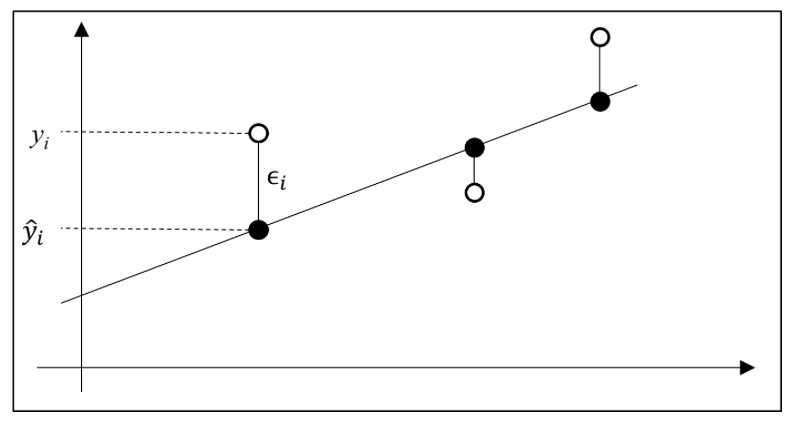
\includegraphics[width=0.5\linewidth]{images/regression.png}
\end{center}
\begin{center}
    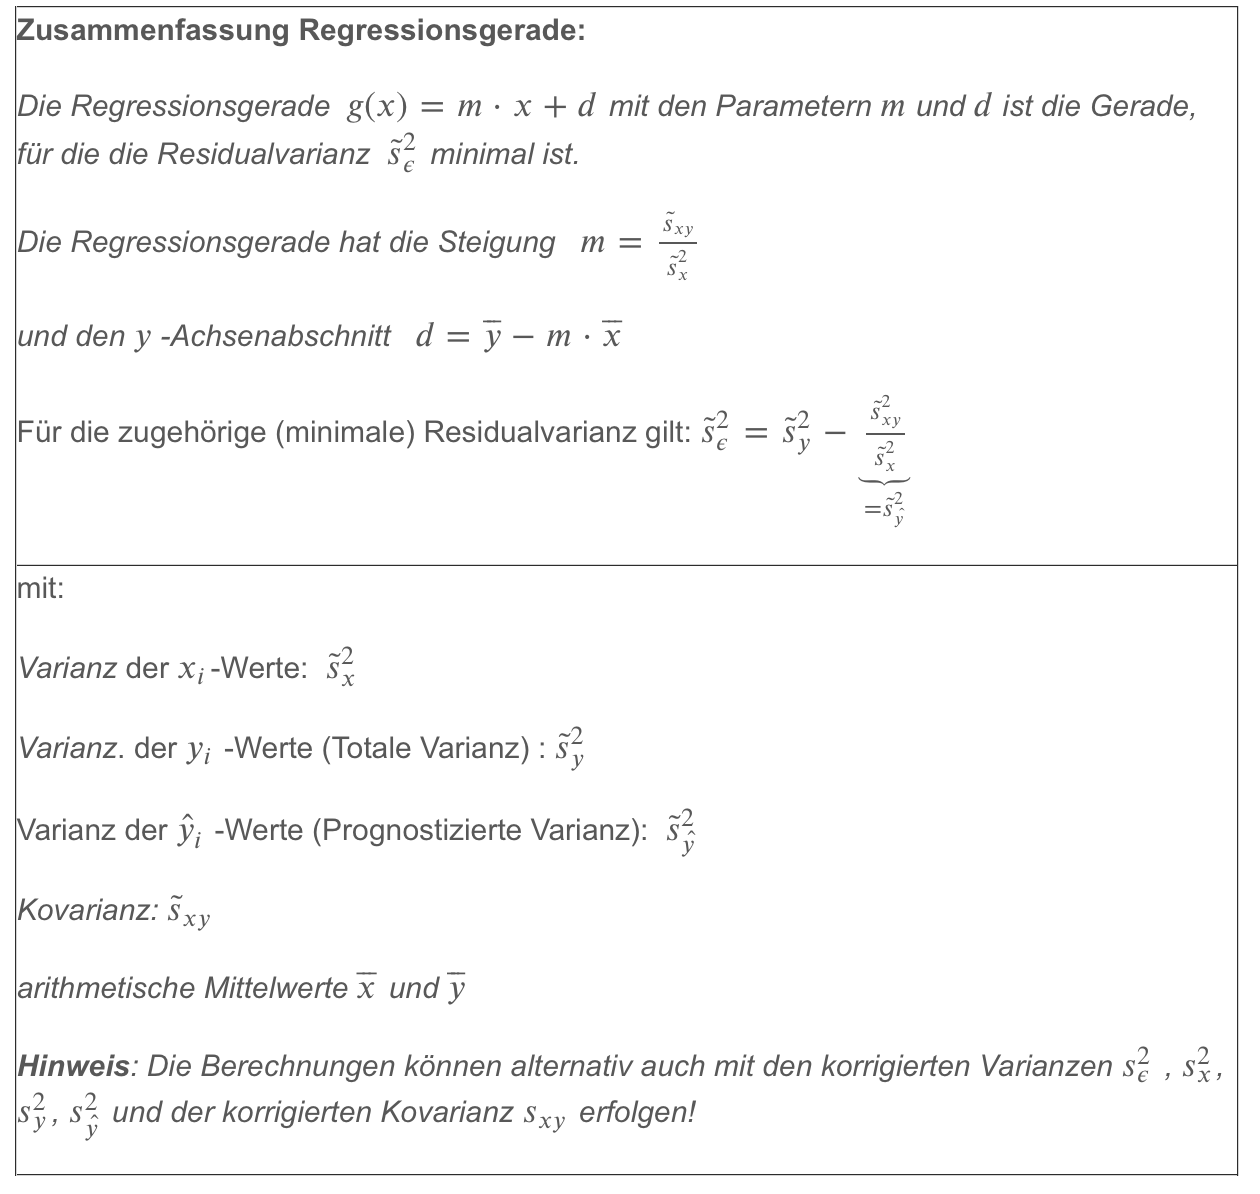
\includegraphics[width=1\linewidth]{images/regression2.png}
\end{center}
\begin{center}
    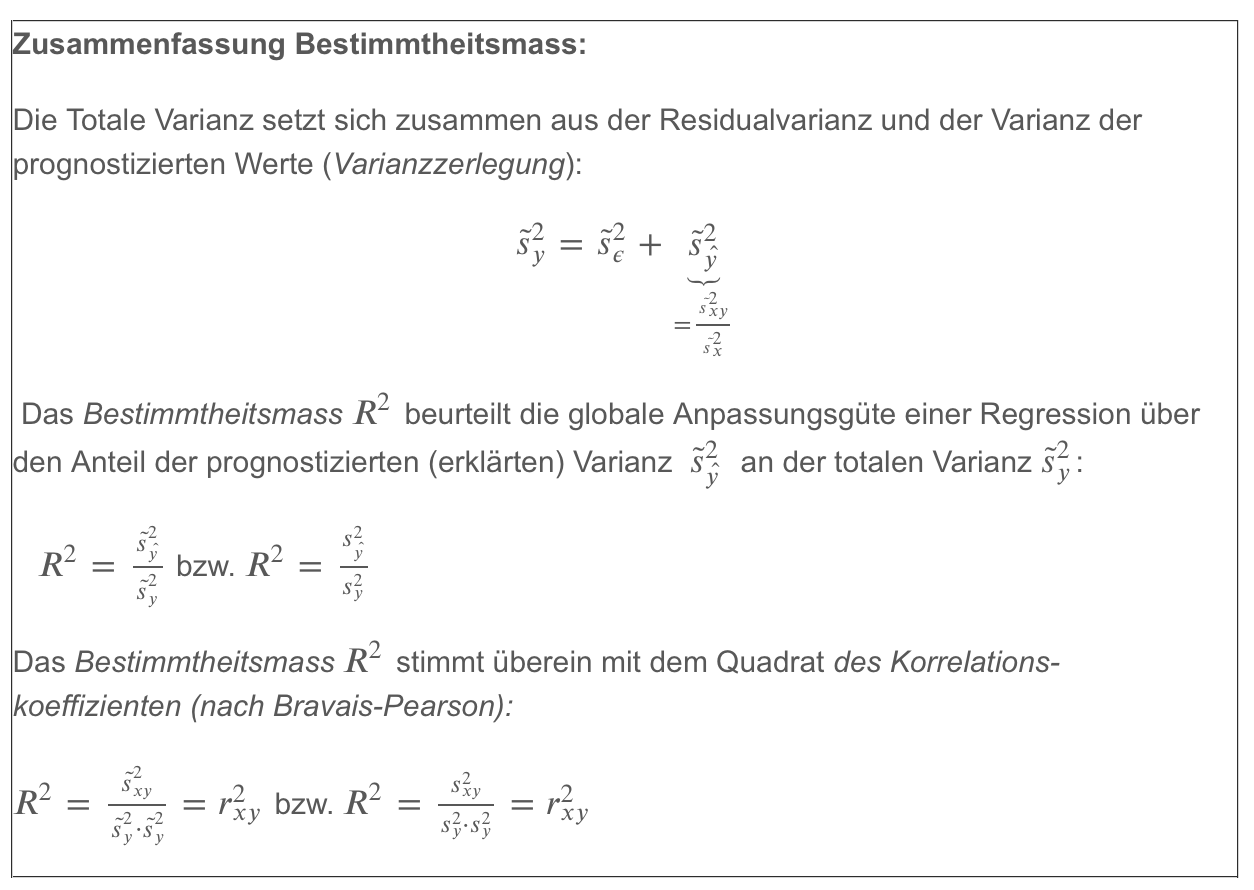
\includegraphics[width=1\linewidth]{images/regression3.png}
\end{center}
\subsection{Bestimmung der Regressionsgeraden als Matrizenproblem}
\label{sec:regressionsgerade}
Die Parameter $m$ und $d$ werden mit der Matrix $A = \begin{pmatrix} x_1 & 1 \\ x_2 & 1 \\ \vdots & \vdots \\ x_n & 1 \end{pmatrix}$ aus den folgenden Normalengleichungen berechnet:
\begin{equation*}
    A^T A \cdot \begin{pmatrix} m \\ d \end{pmatrix} = A^T \cdot \begin{pmatrix} y_1 \\ y_2 \\ \vdots \\ y_n \end{pmatrix}
\end{equation*}
\begin{center}
    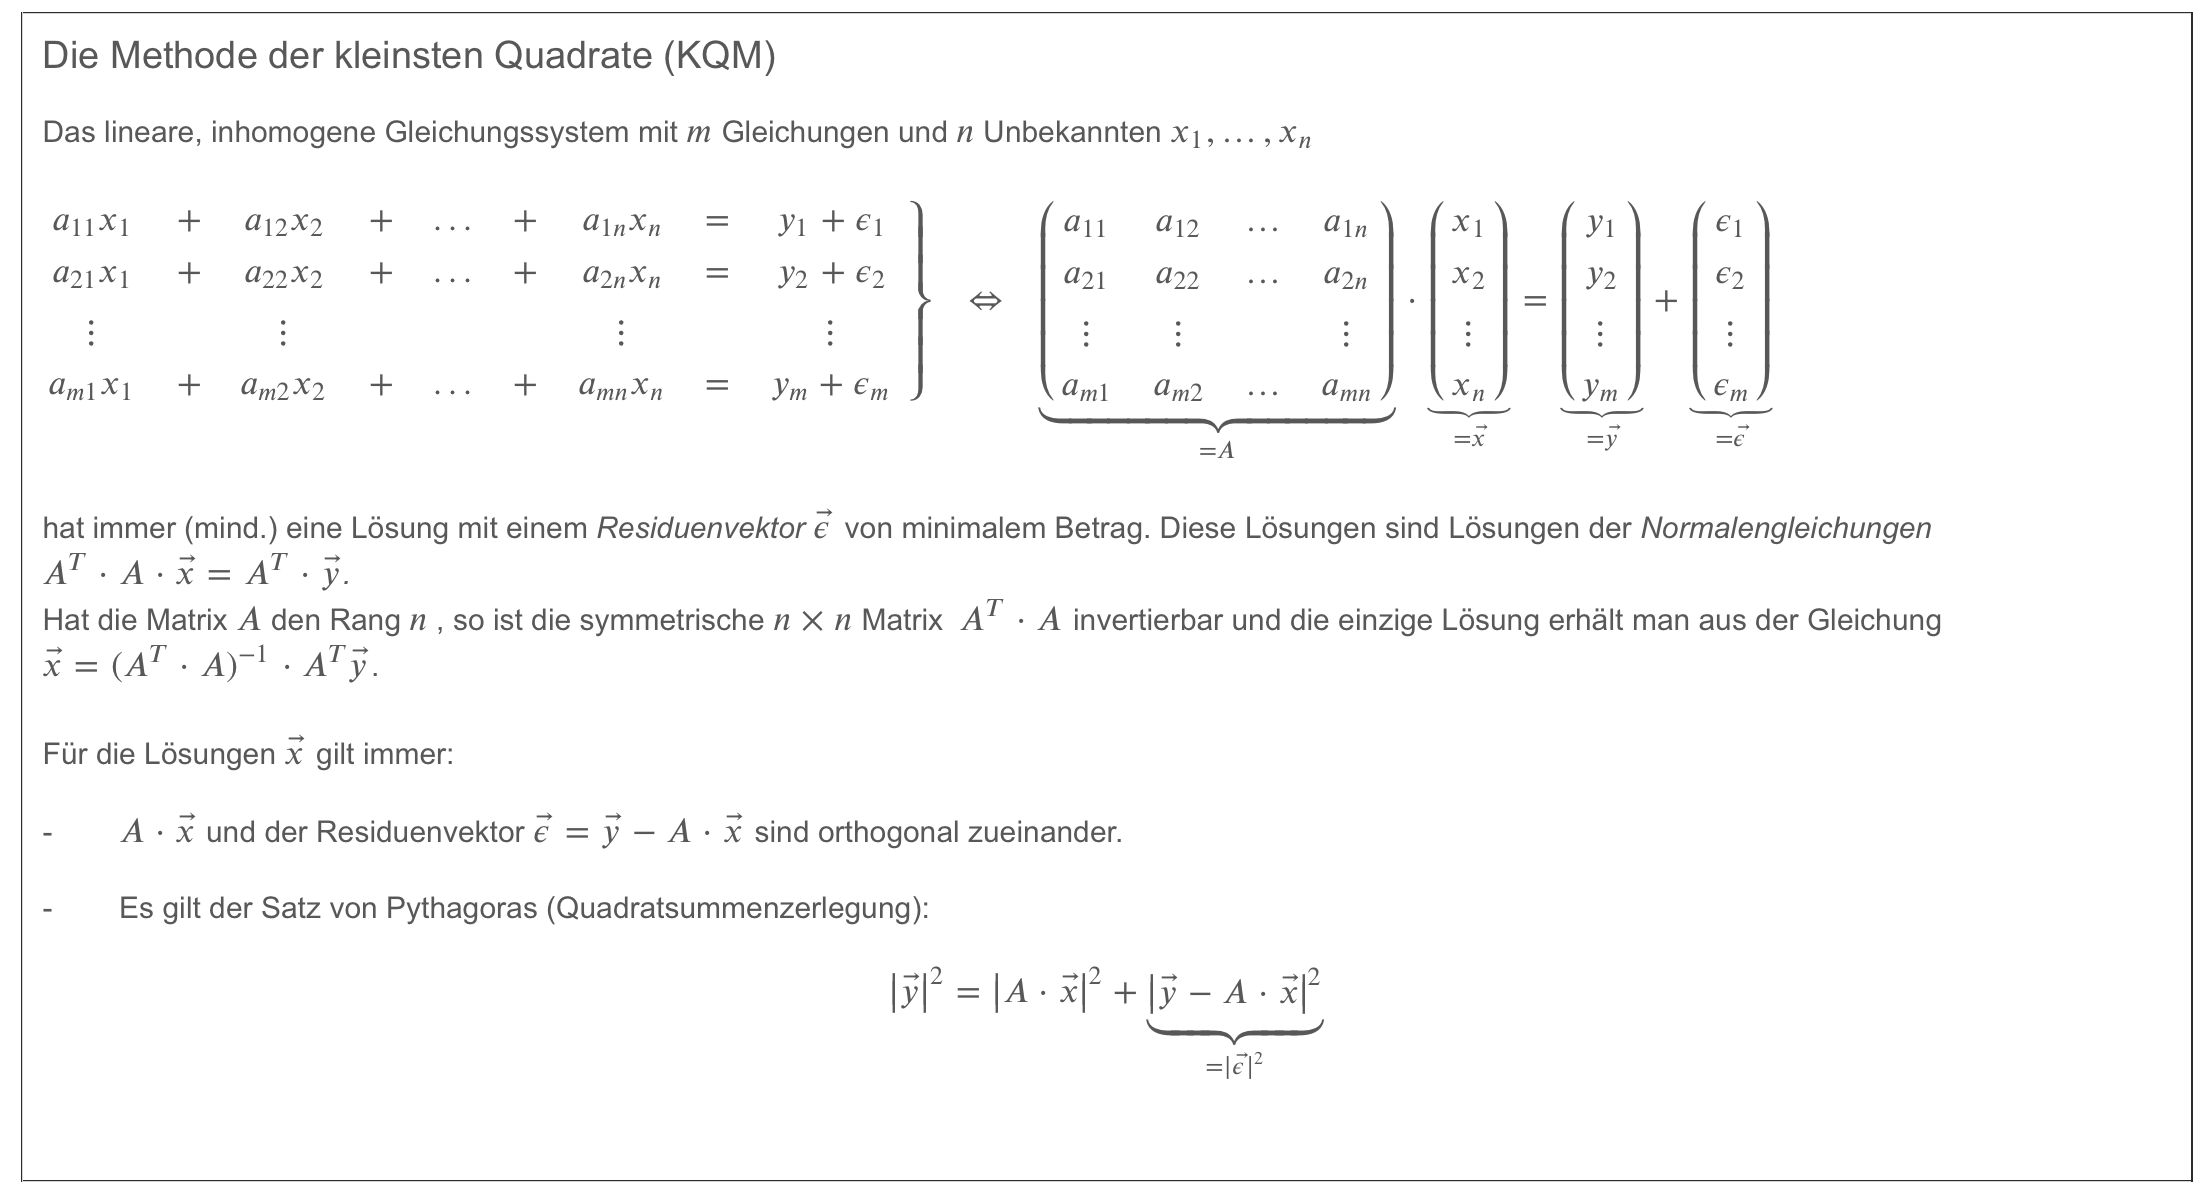
\includegraphics[width=1\linewidth]{images/regression4.png}
\end{center}